\subsection{Theoretische Grundlagen}
\begin{figure}[h!]
  \centering
  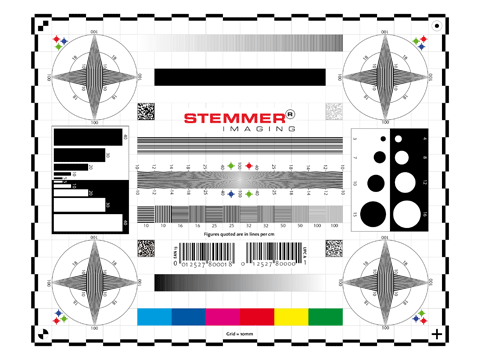
\includegraphics[width=.8\textwidth]{Posten_5_Stemmer}
  \caption{STEMMER IMAGING Test Chart for Machine Vision \cite{ref:stemmer}}
  \label{fig:p5stemmer}
\end{figure}

Die in Abbildung \ref{fig:p5stemmer} dargestellte Testchart bietet verschiedene Merkmale zur Erfassung
der Performance eines optischen Systems.
Die Chart ist mit einem $10\;\text{mm}\; \mathrm{x}\; 10\;\text{mm}$ Gitter versehen, dieses sowie die Balken links und die Kreise rechts sind zur Kalibrierung vorgesehen.

Im unteren Bereich der Chart ist ein Balken mit einem Graustufenverlauf (engl. grayscale bar).
Dieser kann verwendet werden um die Bit-Tiefe der Kamera zu bestimmen und zum Abgleich des Dynamikumfangs.

Die Barcodes (1D und 2D) sind bei diesem Versuch uninteressant.

Wichtiger sind die Quadrate mit den Strichmustern, welche mit der Anzahl Linien beschriftet sind.
Mit diesen können die Auflösung der Linse und des Bildsensors bestimmt werden.
Zum gleichen Zweck wurden die gleich darüber liegenden, zusammenlaufenden Linien angebracht.
Zusammen mit den Kompassrosen ähnlichen Segmenten in den Ecken,
kann die Performance des Linsensystems auf und abseits der optischen Achse verglichen werden.

Das Auflösungsvermögen der Optik und damit die Qualität der Linse wird durch die Modulationstransferfunktion beschrieben. Die Modulation entspricht dem Michelson Kontrast und ist folgendermassen definiert:
\begin{equation}
  M=\frac{I_{max}-I_{min}}{I_{max}+I_{min}}
\end{equation}

Die Modulationstransferfunktion ist definiert als die Abbildung von M durch das Objektiv:
\begin{equation}
  MTF=\frac{M_{Bild}}{M_{Objekt}}
\end{equation}

\newpage
\subsection{Versuchsaufbau}
Benötigtes Material:
\begin{itemize}
\item Kamera Sony DFW-X710
\item Objektiv 12.5mm
\item Testchart Stemmer-Imaging
\item Kamera Samsung Galaxy S6
\end{itemize}



\subsection{Ergebnisse}
\subsubsection{Kamera Sony DFW-X710}
\begin{figure}[h!]
  \centering
  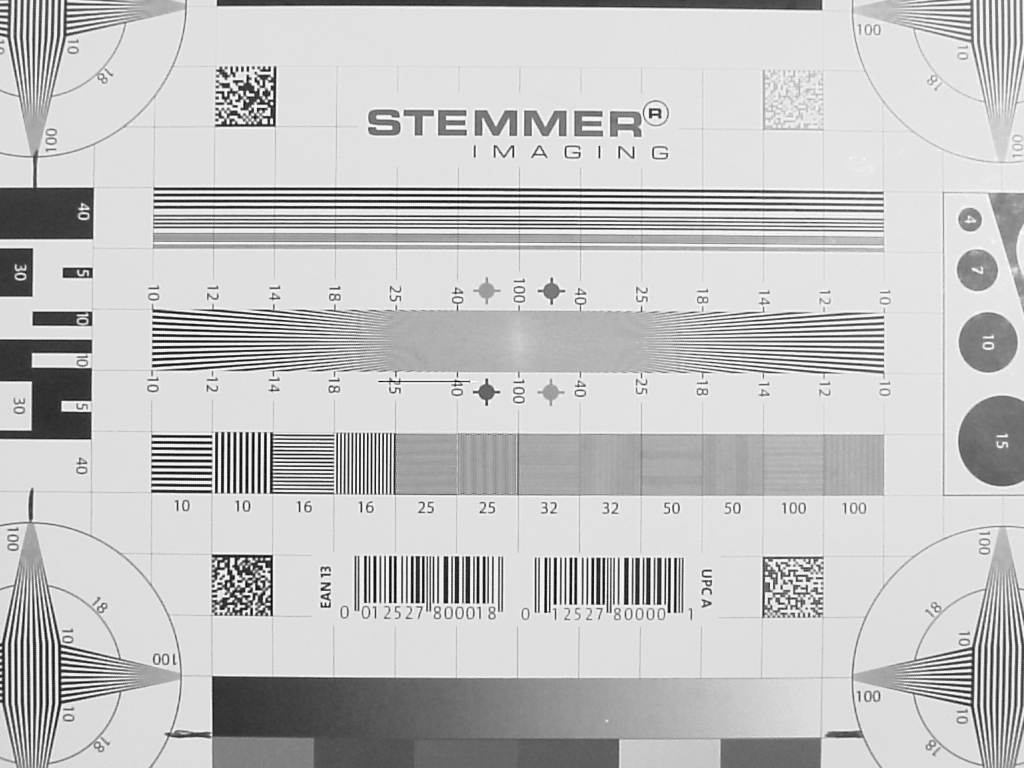
\includegraphics[width=.6\textwidth]{Posten_5_Not_so_rainbow_dildos_0}
  \caption{Graustufenbild mit Sony DFW-X710}
  \label{fig:p5g}
\end{figure}

\begin{table}[h!]
  \centering
  \begin{tabular}{l | l | l }
    Linien/10mm & Horizontal MTF &  Vertikal MTF \\\hline
    10 & 0.937 & 0.976 \\
    16 & 0.851 & 0.867 \\
    25 & 0.282 & 0.518\\
    32 & 0.169 & 0.216 \\
    50 & 0.298 & 0.200 \\
    100 & 0.271 & 0.278 \\
  \end{tabular}
\end{table}

Bei der Tabelle ist zu beachten, dass bei mehr als $\approx$25 Linien das Nyquist-Theorem verletzt wird. Die Linse ist ab diesem Punkt nicht mehr die dominierende Fehlerquelle.

\begin{figure}[H]
  \centering
  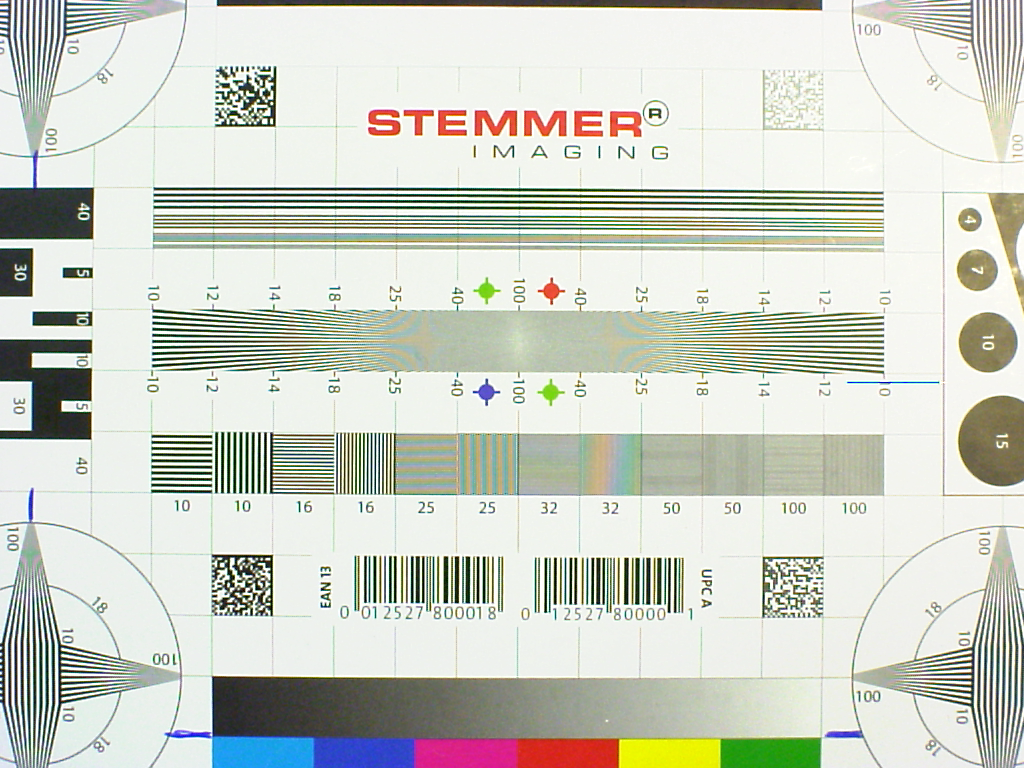
\includegraphics[width=.6\textwidth]{Posten_5_Rainbow_dildos_1}
  \caption{Farbaufname mit Sony DFW-X710}
  \label{fig:p5c}
\end{figure}

Wie in Abbildung \ref{fig:p5c} ersichtlich, sind die durch chromatische Abberation verursachten Fehler bei den Gittern mit 25 und 32 Linien durch die regebogenartige Färbung erkennbar.

\subsubsection{Kamera Samsung Galaxy S6}
\begin{figure}[h!]
  \centering
  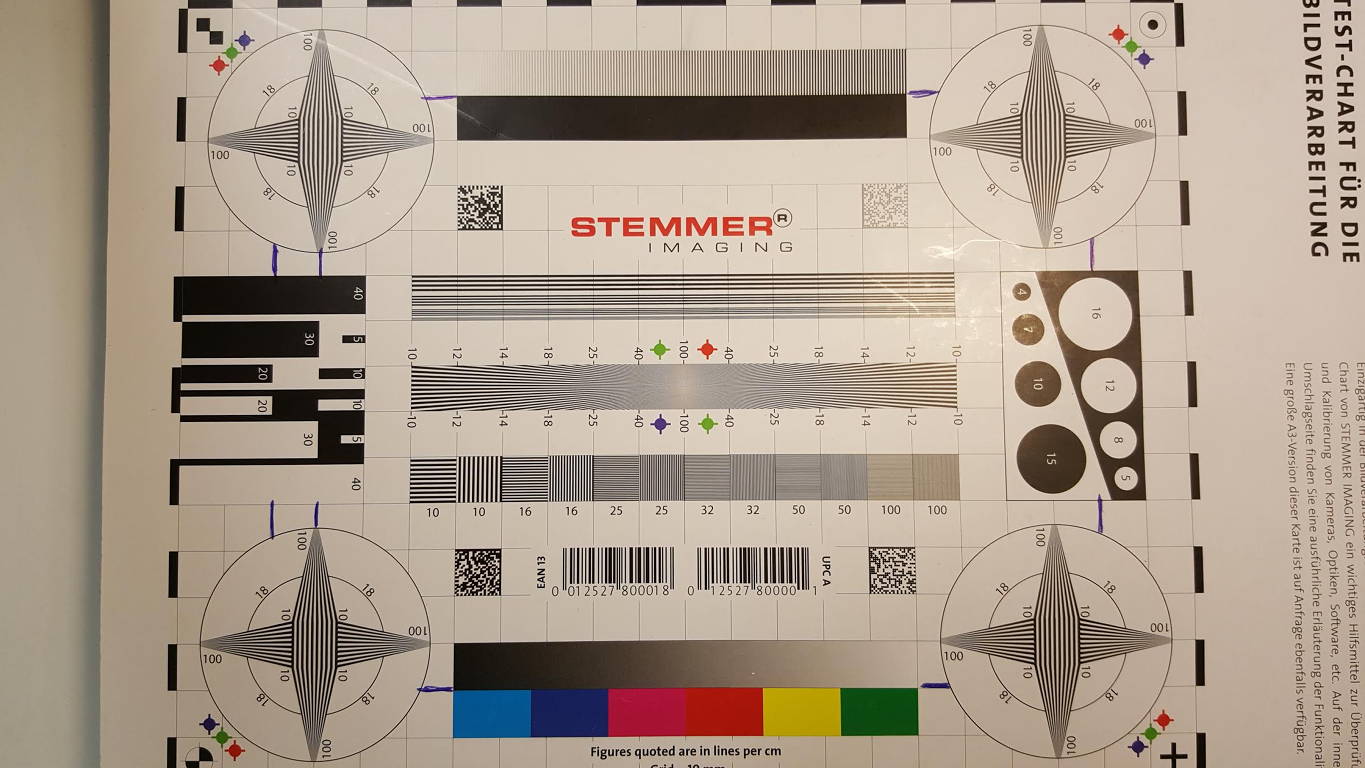
\includegraphics[width=.6\textwidth]{Posten_5_Rainbow_dildos_S6}
  \caption{Farbaufnahme mit Samsung Galaxy S6}
  \label{fig:p5s}
\end{figure}

\begin{table}[h!]
  \centering
  \begin{tabular}{l | l | l }
    Linien/10mm & Horizontal MTF &  Vertikal MTF \\\hline
    10 & 1 &  1\\
    16 & 1 & 0.992\\
    25 & 0.612 & 0.742 \\
    32 & 0.275 & 0.447 \\
    50 & 0.254 & 0.267 \\
    100 & 0.243 & 0.361 \\
  \end{tabular}
\end{table}

\newpage
\subsection{Erkenntnisse}
Wird die chromatische Abberation betrachtet, scheint die Handy Kamera deutlich besser zu sein.
Dies ist wenig erstaunlich, denn das Linsensystem beim Handy ist wesentlich kleiner, die Zahl der Fehlerquellen dementsprechend klein. Nachteile der Handy Kamera sind aber in anderen Bereichen (Zoom/Schärfentiefe) zu finden.

Zu berücksichtigen ist, dass die Aufnahm mit dem Handy nur bedingt für die Analyse der Bildqualität geeignet ist.
Die Kamera kann nur Bilder im JPEG-Format speichern, dieses reduziert die Bildgrösse
durch verlustbehaftete Komprimierung. Die Ursache eines Abbildungsfehlers kann sowohl im Optischensystem, wie auch in der digitalen Verarbeitung zu finden sein.

\begin{figure}[h!]
  \centering
  \begin{subfigure}[t]{0.49\textwidth}
    \centering
    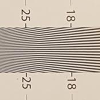
\includegraphics[width=.8\textwidth]{Posten_5_Rainbow_dildos_XXL_S6}
    \caption{JPEG komprimierte Aufnahme (Galaxy S6)}
  \end{subfigure}
  %
  \begin{subfigure}[t]{0.49\textwidth}
    \centering
    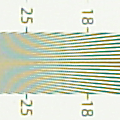
\includegraphics[width=.8\textwidth]{Posten_5_Rainbow_dildos_XXL}
    \caption{Verlustlose Aufnahme (Sony DFW-X710)}
  \end{subfigure}
  %
  \caption{Vergleich verlustbehaftete und verlustlose Kompression}
  \label{fig:p5sc}
\end{figure}

In Abbildung \ref{fig:p5sc} sind die für JPEG typischen Bildstörung besonders gut bei den Zahlen ersichtlich.

Des weiteren scheinen die Linien kurz vor der 25-er Marke die Richtung zu ändern,
ein Effekt welcher für Abtastfehler typisch ist. Der selbe Effekt tritt bei der Sony Kamera nur wenig später auf. Dies ist durch die begrenzte Auflösung erklärbar.

